\documentclass[dvipdfmx]{beamer}

\usepackage{graphics}
\usepackage{amsmath}
\usepackage{amssymb}
\usepackage{ascmac}
\usepackage{txfonts}
\usepackage{bm}
\usepackage{docmute}
\usepackage{tikz}
\usetikzlibrary{calc}
\usetikzlibrary{intersections}

\usetheme{Madrid}
\usefonttheme{professionalfonts}


\title{三角形の合同}
\author{近藤綜太}

\begin{document}
	\maketitle
	\begin{frame}{問題}
		次の図で $\triangle \mathrm{ABC}$は $\angle ABC=90^\circ$の直角二等辺三角形である.
		$A, C$から直線 $m$に下した垂線の交点をそれぞれ $D, E$とする. $AD=BE$を証明せよ.
		\begin{figure}[htbp]
			\centering
			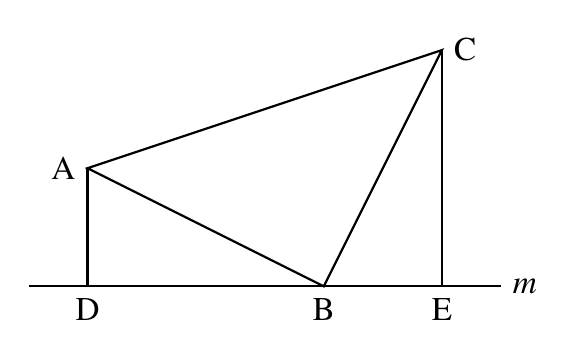
\begin{tikzpicture}[scale=1.5]\large

				\coordinate(a) at (0, 1);
				\coordinate(b) at (2, 0);
				\coordinate(c) at (3, 2);
				\coordinate(d) at (0, 0);
				\coordinate(e) at (3, 0);

				\draw[semithick] (-0.5, 0)--(3.5, 0)node[right]{ $m$ };
				\draw[thick] (a)node[left]{A}--(b)node[below]{B}--(c)node[right]{C}--cycle;
				\draw[thick] (a)--(d)node[below]{D};
				\draw[thick] (c)--(e)node[below]{E};
			\end{tikzpicture}
			\caption{問題}
			\label{tikz:question}
		\end{figure}
	\end{frame}

	\begin{frame}{方針}
		\begin{columns}
			\begin{column}{0.4\textwidth}
		\begin{figure}[htbp]
			\centering
					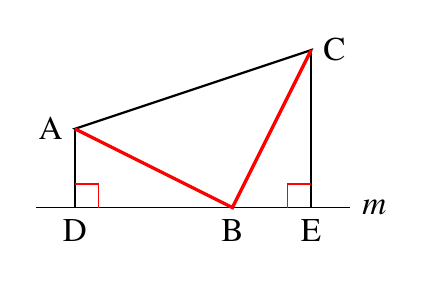
\begin{tikzpicture}[scale=1]\large

						\coordinate(a) at (0, 1);
						\coordinate(b) at (2, 0);
						\coordinate(c) at (3, 2);
						\coordinate(d) at (0, 0);
						\coordinate(e) at (3, 0);

						\draw[semithick] (-0.5, 0)--(3.5, 0)node[right]{ $m$ };
						\draw[thick] (a)node[left]{A}--(b)node[below]{B}--(c)node[right]{C}--cycle;
						\draw[thick] (a)--(d)node[below]{D};
						\draw[thick] (c)--(e)node[below]{E};

						\draw[very thick, red](a)--(b)--(c);
						\draw[semithick, red](0, 0.3)--(0.3, 0.3)--(0.3, 0);
						\draw[semithick, red]($(0, 0.3)+(e)$)--($(-0.3, 0.3)+(e)$)--($(e)+(-0.3, 0)$);
					\end{tikzpicture}
				\end{figure}
			\end{column}

			\begin{column}{0.6\textwidth}
				% \pause
				$\triangle\mathrm{ADB}\equiv\triangle\mathrm{BEC}$を証明する.
				% \pause
				\begin{itemize}
					\item $\mathrm{AB=BC}$が二等辺三角形からわかる.
				% \pause
					\item $\angle\mathrm{ADB}=\angle\mathrm{BEC}=90^\circ$
				\end{itemize}
				% \pause
				直角三角形の斜辺がわかっている.
				そこで次のどちらかが分かれば良い.
				% \pause
				\begin{itemize}
					\item 直角ではない角が1組等しいこと
					\item 斜辺以外の辺の長さが1組等しいこと
				\end{itemize}
			\end{column}
		\end{columns}
	\end{frame}

	\begin{frame}{同じ角度の引き算}
		方針から辺の長さを考えるのが難しいと分かれば,
		角度で何とかしようと考える. 
		$\angle\mathrm{CBE}$を計算することを考える.
		これは2通りの計算が考えられるはずだ.

		\begin{columns}
			\begin{column}{0.4\textwidth}
				\begin{figure}[htbp]
					\centering
					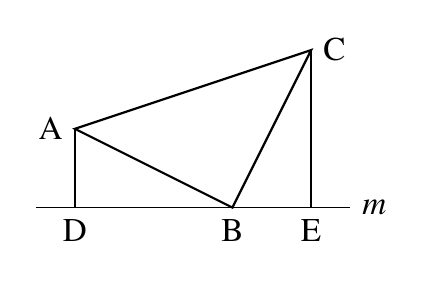
\begin{tikzpicture}[scale=1]\large

						\coordinate(a) at (0, 1);
						\coordinate(b) at (2, 0);
						\coordinate(c) at (3, 2);
						\coordinate(d) at (0, 0);
						\coordinate(e) at (3, 0);

						\draw[semithick] (-0.5, 0)--(3.5, 0)node[right]{ $m$ };
						\draw[thick] (a)node[left]{A}--(b)node[below]{B}--(c)node[right]{C}--cycle;
						\draw[thick] (a)--(d)node[below]{D};
						\draw[thick] (c)--(e)node[below]{E};

					\end{tikzpicture}
				\end{figure}
			\end{column}

			\begin{column}{0.6\textwidth}
		% \pause
				\begin{itemize}
					\item 直線 $m$による式
						\begin{align*}
						\angle\mathrm{CBE}&=180^\circ - \angle\mathrm{ABC}-\angle\mathrm{ABD}\\
										  &= 90^\circ  -\angle\mathrm{ABD}
						\end{align*}
		% \pause
					\item 三角形の内角の和が $180^\circ$による式
						\begin{align*}
						\angle\mathrm{CBE}&=180^\circ - \angle\mathrm{CEB}-\angle\mathrm{BCE}\\
										  &= 90^\circ  -\angle\mathrm{BCE}
						\end{align*}
				\end{itemize}
			\end{column}
		\end{columns}
		% \pause

		これで,1組の等しい角が見つかった.

		
	\end{frame}


	\begin{frame}{解答例(前半)}
		$\triangle\mathrm{ABD}$と$\triangle\mathrm{BCE}$において,\\
		% \pause
		仮定より,
		\[\angle\mathrm{ADB}=\angle\mathrm{BEC}=90^\circ\qquad \cdots (1)\]
		% \pause
		$\triangle\mathrm{ABC}$が $\mathrm{BA=BC}$の二等辺三角形より,
		\[\mathrm{AB=BC}\qquad \cdots (2)\]
		% \pause
		直線 $m$においては以下の式が成立する.
		\begin{align*}
		\angle\mathrm{CBE}=180^\circ - \angle\mathrm{ABC}-\angle\mathrm{ABD}
						  = 90^\circ  -\angle\mathrm{ABD}
		\end{align*}
		% \pause
		また,$\triangle\mathrm{BCE}$において,三角形の内角の和が $180^\circ$より,
		\begin{align*}
		\angle\mathrm{CBE}=180^\circ - \angle\mathrm{CEB}-\angle\mathrm{BCE}
						  = 90^\circ  -\angle\mathrm{BCE}
		\end{align*}
		% \pause
		\[\therefore \angle\mathrm{ABD}= \angle\mathrm{BCE}\qquad \cdots(3)\]
	\end{frame}

	\begin{frame}{解答例(後半)}
		$(1), (2), (3)$より,直角三角形の斜辺と1つの鋭角がそれぞれ等しいので,
		\[\triangle\mathrm{ADB}\equiv\triangle\mathrm{BEC}\]
		% \pause
		合同な三角形の対応する辺は等しいので,
		\[\mathrm{AD=BE}\quad\Box\]
	\end{frame}

	\begin{frame}{余談}
		
		\begin{columns}
			\begin{column}{0.4\textwidth}
				\begin{figure}[htbp]
					\centering
					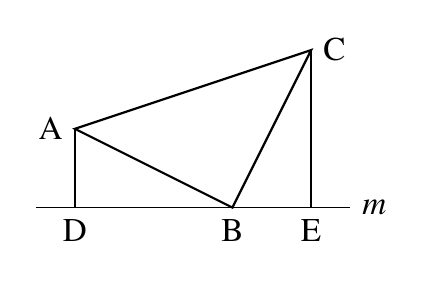
\begin{tikzpicture}[scale=1]\large

						\coordinate(a) at (0, 1);
						\coordinate(b) at (2, 0);
						\coordinate(c) at (3, 2);
						\coordinate(d) at (0, 0);
						\coordinate(e) at (3, 0);

						\draw[semithick] (-0.5, 0)--(3.5, 0)node[right]{ $m$ };
						\draw[thick] (a)node[left]{A}--(b)node[below]{B}--(c)node[right]{C}--cycle;
						\draw[thick] (a)--(d)node[below]{D};
						\draw[thick] (c)--(e)node[below]{E};

					\end{tikzpicture}
				\end{figure}
			\end{column}

			\begin{column}{0.6\textwidth}
				左の図を使うと三平方の定理を証明することができる.
				これは第20代アメリカ大統領の\\
				ジェームズ・A・ガーフィールド\\
				が発表したものだ.


				台形の面積を公式と,3つの三角形の和との2つの方法で表すことで
				等式を作ると証明できる.

				各自でやってみるとよい.
			\end{column}
		\end{columns}


	\end{frame}

	\begin{frame}{余談}
		きれいなスライドを作るのは最初だけ.以降は手書きの回答を
		表示します.

		来週以降は,参加者がそれなりにいそうならやります.
		問題はみんなから集めるつもりです.なければ僕が用意します.

	\end{frame}


\end{document}
